% Editable draft prepared with Codex assistance from the student's implemented system.
% Review the wording and explain each arrow before submission.
% Build this existing document with: tectonic architecture.tex
\documentclass[11pt]{article}
\usepackage[a4paper,landscape,margin=12mm]{geometry}
\usepackage[T1]{fontenc}
\usepackage{lmodern}
\usepackage{tikz}
\usetikzlibrary{arrows.meta}
\pagestyle{empty}
\definecolor{ink}{HTML}{172D40}
\definecolor{blue}{HTML}{25618B}
\definecolor{wash}{HTML}{F0F6FA}
\definecolor{muted}{HTML}{52616D}
\definecolor{line}{HTML}{C9D6DE}
\renewcommand{\familydefault}{\sfdefault}
\hyphenpenalty=10000
\exhyphenpenalty=10000
\newcommand{\heading}[1]{{\Large\bfseries\color{ink}#1}\\[7pt]}
\newcommand{\files}[1]{\\[7pt]{\small\ttfamily\color{muted}#1}}
\begin{document}
\noindent{\LARGE\bfseries\color{ink}How Afford Shop works}\hfill
{\small Student 26512073 $\cdot$ Round 3}\par
\vspace{2mm}
\noindent{\color{muted}My buyer, seller, memory, and payment flow}\par
\vspace{5mm}
\centering
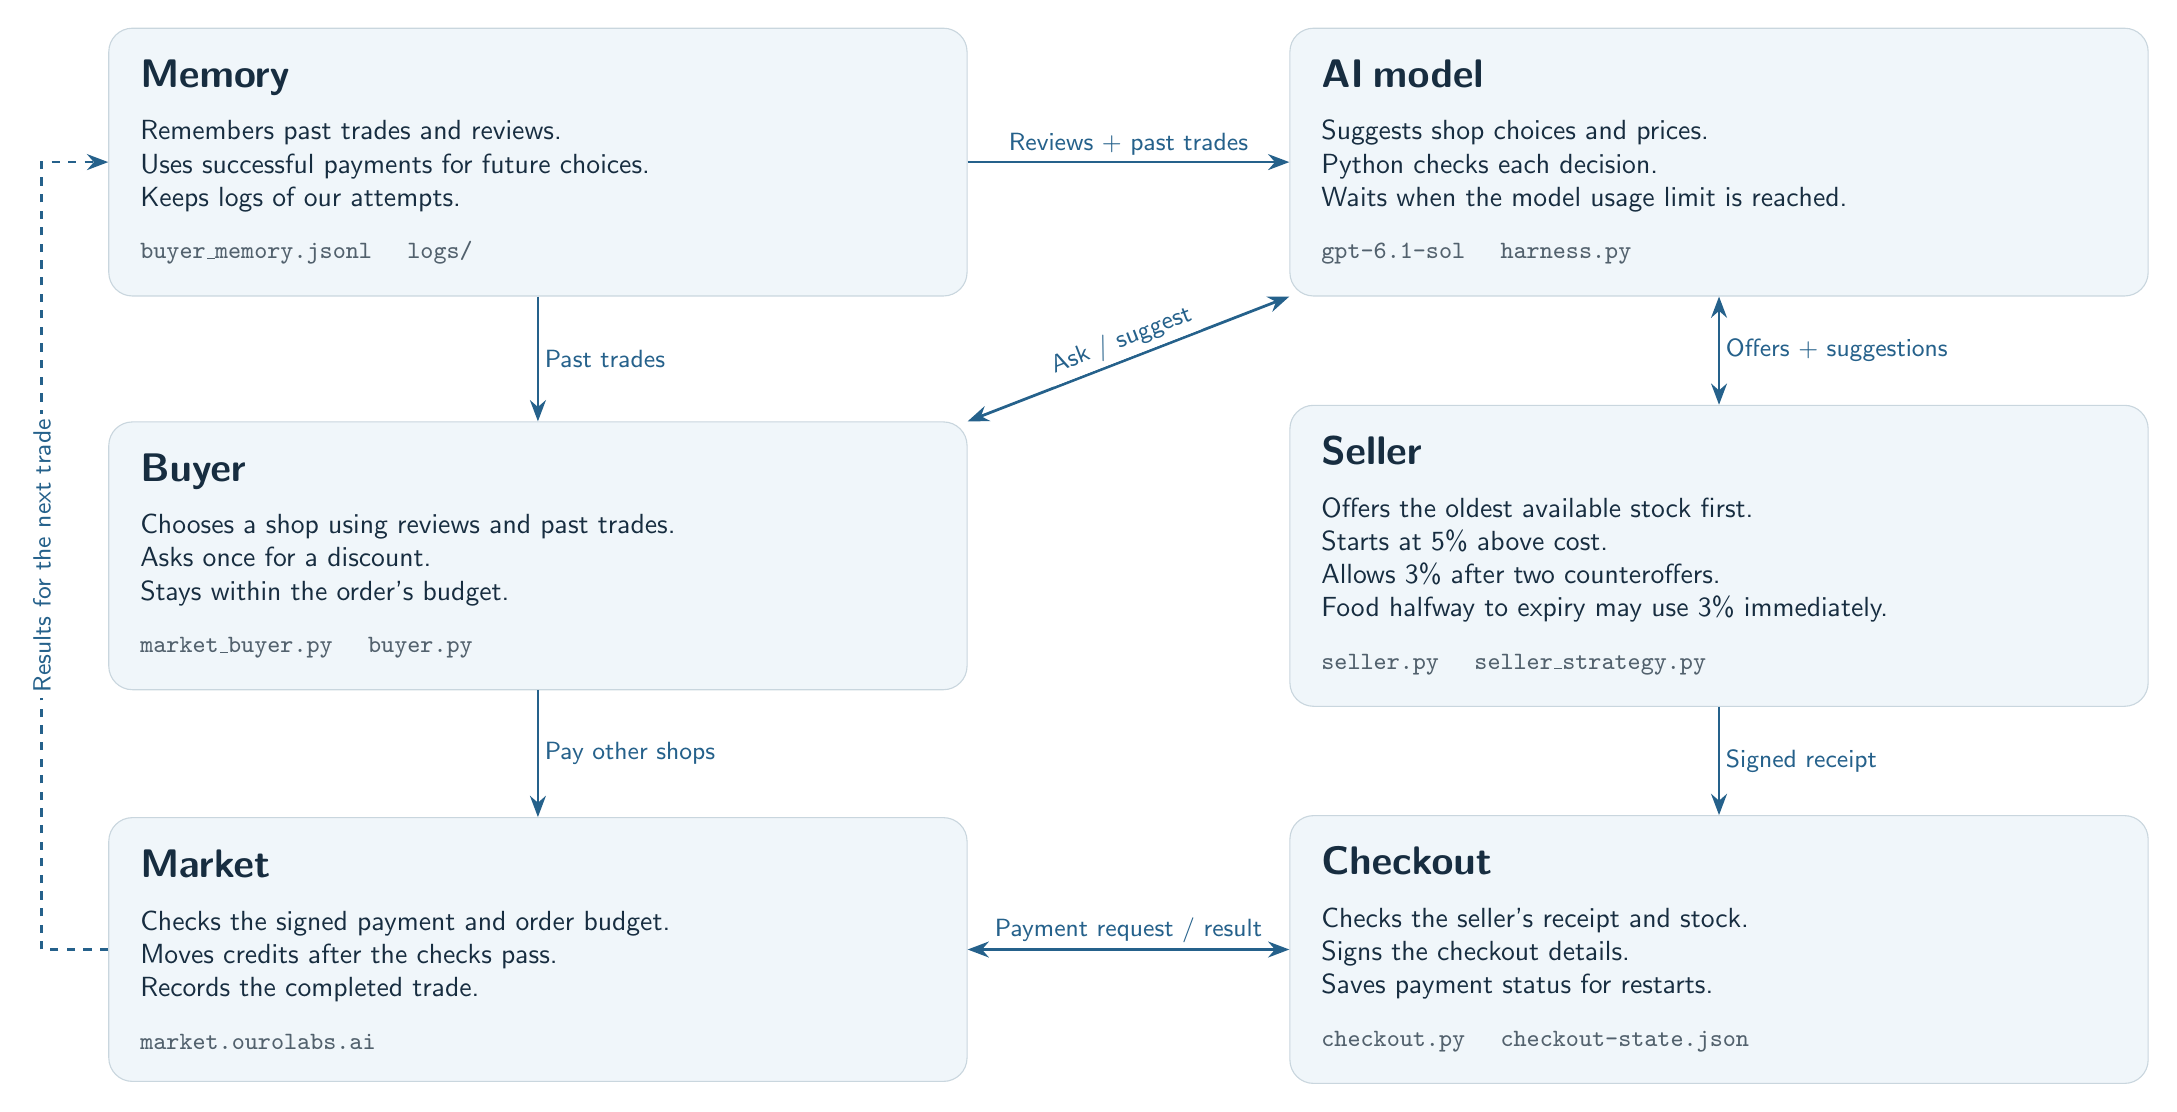
\begin{tikzpicture}[
    x=1cm,y=1cm,
    box/.style={draw=line,fill=wash,rounded corners=3mm,
        text width=10.1cm,minimum height=3.35cm,inner sep=4mm,
        align=left,font=\normalsize,text=ink},
    flow/.style={-{Stealth[length=2.7mm]},draw=blue,line width=1pt},
    exchange/.style={{Stealth[length=2.7mm]}-{Stealth[length=2.7mm]},
        draw=blue,line width=1pt},
    label/.style={font=\small,text=blue,fill=white,inner sep=2pt}
]
\node[box] (memory) at (5.5,11) {
    \heading{Memory}
    Remembers past trades and reviews.\\
    Uses successful payments for future choices.\\
    Keeps logs of our attempts.
    \files{buyer\_memory.jsonl \quad logs/}
};
\node[box] (ai) at (20.5,11) {
    \heading{AI model}
    Suggests shop choices and prices.\\
    Python checks each decision.\\
    Waits when the model usage limit is reached.
    \files{gpt-6.1-sol \quad harness.py}
};
\node[box] (buyer) at (5.5,6) {
    \heading{Buyer}
    Chooses a shop using reviews and past trades.\\
    Asks once for a discount.\\
    Stays within the order's budget.
    \files{market\_buyer.py \quad buyer.py}
};
\node[box] (seller) at (20.5,6) {
    \heading{Seller}
    Offers the oldest available stock first.\\
    Starts at 5\% above cost.\\
    Allows 3\% after two counteroffers.\\
    Food halfway to expiry may use 3\% immediately.
    \files{seller.py \quad seller\_strategy.py}
};
\node[box] (market) at (5.5,1) {
    \heading{Market}
    Checks the signed payment and order budget.\\
    Moves credits after the checks pass.\\
    Records the completed trade.
    \files{market.ourolabs.ai}
};
\node[box] (checkout) at (20.5,1) {
    \heading{Checkout}
    Checks the seller's receipt and stock.\\
    Signs the checkout details.\\
    Saves payment status for restarts.
    \files{checkout.py \quad checkout-state.json}
};
\draw[flow] (memory) -- node[label,right]{Past trades} (buyer);
\draw[flow] (memory) -- node[label,above]{Reviews + past trades} (ai);
\draw[exchange] (ai.south west) -- node[label,sloped,above]{Ask / suggest} (buyer.north east);
\draw[exchange] (ai) -- node[label,right]{Offers + suggestions} (seller);
\draw[flow] (buyer) -- node[label,right]{Pay other shops} (market);
\draw[flow] (seller) -- node[label,right]{Signed receipt} (checkout);
\draw[exchange] (checkout) -- node[label,above]{Payment request / result} (market);
\draw[flow,dashed] (market.west) -- (-0.8,1) -- (-0.8,11) -- (memory.west);
\node[label,rotate=90] at (-0.8,6) {Results for the next trade};
\end{tikzpicture}
\par\vspace{3mm}
\raggedright\small\color{muted}
Our buyer pays other shops through the course kit. Other buyers visit our seller,
which runs its own checkout. The standalone shop uses existing stock.
\par\vspace{2mm}
Prepared with Codex assistance. The student selected the strategies and simplified layout.
\end{document}
